%\documentclass[handout]{beamer} 
\documentclass[t,12pt,numbers,fleqn]{beamer}
%\documentclass[ignorenonframetext]{beamer}

\newif\ifquestions
%\questionstrue
\questionsfalse

\usepackage{pgfpages} 
\usepackage{hyperref}
\hypersetup{colorlinks=true,
    linkcolor=blue,
    citecolor=blue,
    filecolor=blue,
    urlcolor=blue,
    unicode=false}
\urlstyle{same}

\usepackage{booktabs}
\usepackage{multirow}

\bibliographystyle{plain}

%\usetheme{Iimenau}

\useoutertheme{split} %so the footline can be seen, without needing pgfpages

%\pgfpagesuselayout{resize to}[letterpaper,border shrink=5mm,landscape]  %if this is uncommented, the hyperref links do not work

\mode<presentation>{}

\input{../def-beamer}

\newcommand{\topic}{17 Math Review}

%Title page information for 1D04 lectures slides

% Define year specific parameters - used in title page and footer

\newcommand{\season}{Fall} %use to switch between Winter and Fall
\newcommand{\instructor}{Dr.~Spencer Smith} %use to switch instructor
\newcommand{\instructSmall}{Dr.~Smith}
\newcommand{\yr}{2019}
\newcommand{\courseCode}{CAS 741, CES 741}
\newcommand{\courseTitle}{Development of Scientific Computing Software}

%\setbeamerfont{structure}{series=\bfseries}
%\usefonttheme[stillsansseriftext,stillsansserifmath]{serif}
\setbeamertemplate{navigation symbols}{} 
\setbeamertemplate{itemize item}[ball]

\title{
  {\normalsize \bf 
    \borange{\courseCode~(\courseTitle)\\ \season~\yr}}\\[2ex]
  {\Large \bf \topic}}

\author[Smith]{\instructor}

\institute{
  Faculty of Engineering,
  McMaster University}

\date{
\today
%January 2011\\
\bc
  \includegraphics[scale = 0.2, keepaspectratio]
  {../mcmaster-logo-full-color.jpg}
\ec
}

\renewcommand{\borange}[1] %orange is too hard to read
{
   \bred{#1}
}

\begin{document}

\input{../footline}

%%%%%%%%%%%%%%%%%%%%%%%%%%%%%%%%%%%%%%%%%%%%%%%%%%%%%%

\begin{frame}
\frametitle{Math Review}

\bi
\item MG Presentations
\bi
\item Steven
\item Isobel
\ei
\item Administrative details
\item Questions?
\item New Uses Relation for SWHS
\item Math review introduction
\item Review of sets, relations and functions
\item Review of logic
\item Review of types, sets, sequence and tuples
\item Multiple assignment statement
\item Conditional rules
\item Finite state machines
\ei
\end{frame}

%%%%%%%%%%%%%%%%%%%%%%%%%%%%%%%%%%%%%%%%%%%%%%%%%%%%%%

\begin{frame}
\frametitle{Administrative Details}

\bi
\item GitHub issues for colleagues
\bi
\item Assigned 1 colleague (see \texttt{Repos.xlsx} in repo)
\item Provide at least 5 issues on their MG
\item Grading as before
\item Due by Tuesday, Nov 14, 11:59 pm
\ei
\item MG marking scheme in Avenue (soon)
\item Updated MIS template in CAS 741 repo (soon)
\ei

\end{frame}

%%%%%%%%%%%%%%%%%%%%%%%%%%%%%%%%%%%%%%%%%%%%%%%%%%%%%%

\begin{frame}
\frametitle{Administrative Details: Deadlines}
~\newline
\begin{tabular}{l l l}
\textbf{MG} & Week 09 & Nov 8\\
\textbf{MIS Present} & Week 10 & Week of Nov 13\\
\textbf{MIS} & Week 11 & Nov 22\\
Impl.\ Present & Week 12 & Week of Nov 27\\
Final Documentation & Week 13 & Dec 6\\
\end {tabular}

\end{frame}

%%%%%%%%%%%%%%%%%%%%%%%%%%%%%%%%%%%%%%%%%%%%%%%%%%%%%%

\begin{frame}
\frametitle{Administrative Details: Presentation Schedule}

\bi
\item MIS Present
\bi
\item \textbf{Tuesday: Isobel, Keshav, Paul}
\item \textbf{Friday: Shusheng, Xiaoye, Devi}
\ei
\item Impl.\ Present
\bi
\item Tuesday: Alexander S., Steven, Alexandre P.
\item Friday: Jason, Geneva, Yuzhi
\ei

\ei

\end{frame}

%%%%%%%%%%%%%%%%%%%%%%%%%%%%%%%%%%%%%%%%%%%%%%%%%%%%%%

\begin{frame}
\frametitle{Questions?}
\begin{itemize}
\item Questions about Module Guides?
\item Questions about MIS?
\end{itemize}
\end{frame}

%%%%%%%%%%%%%%%%%%%%%%%%%%%%%%%%%%%%%%%%%%%%%%%%%%%%%%

\begin{frame}

\frametitle{Revised Uses Relation for SWHS}

\begin{center}
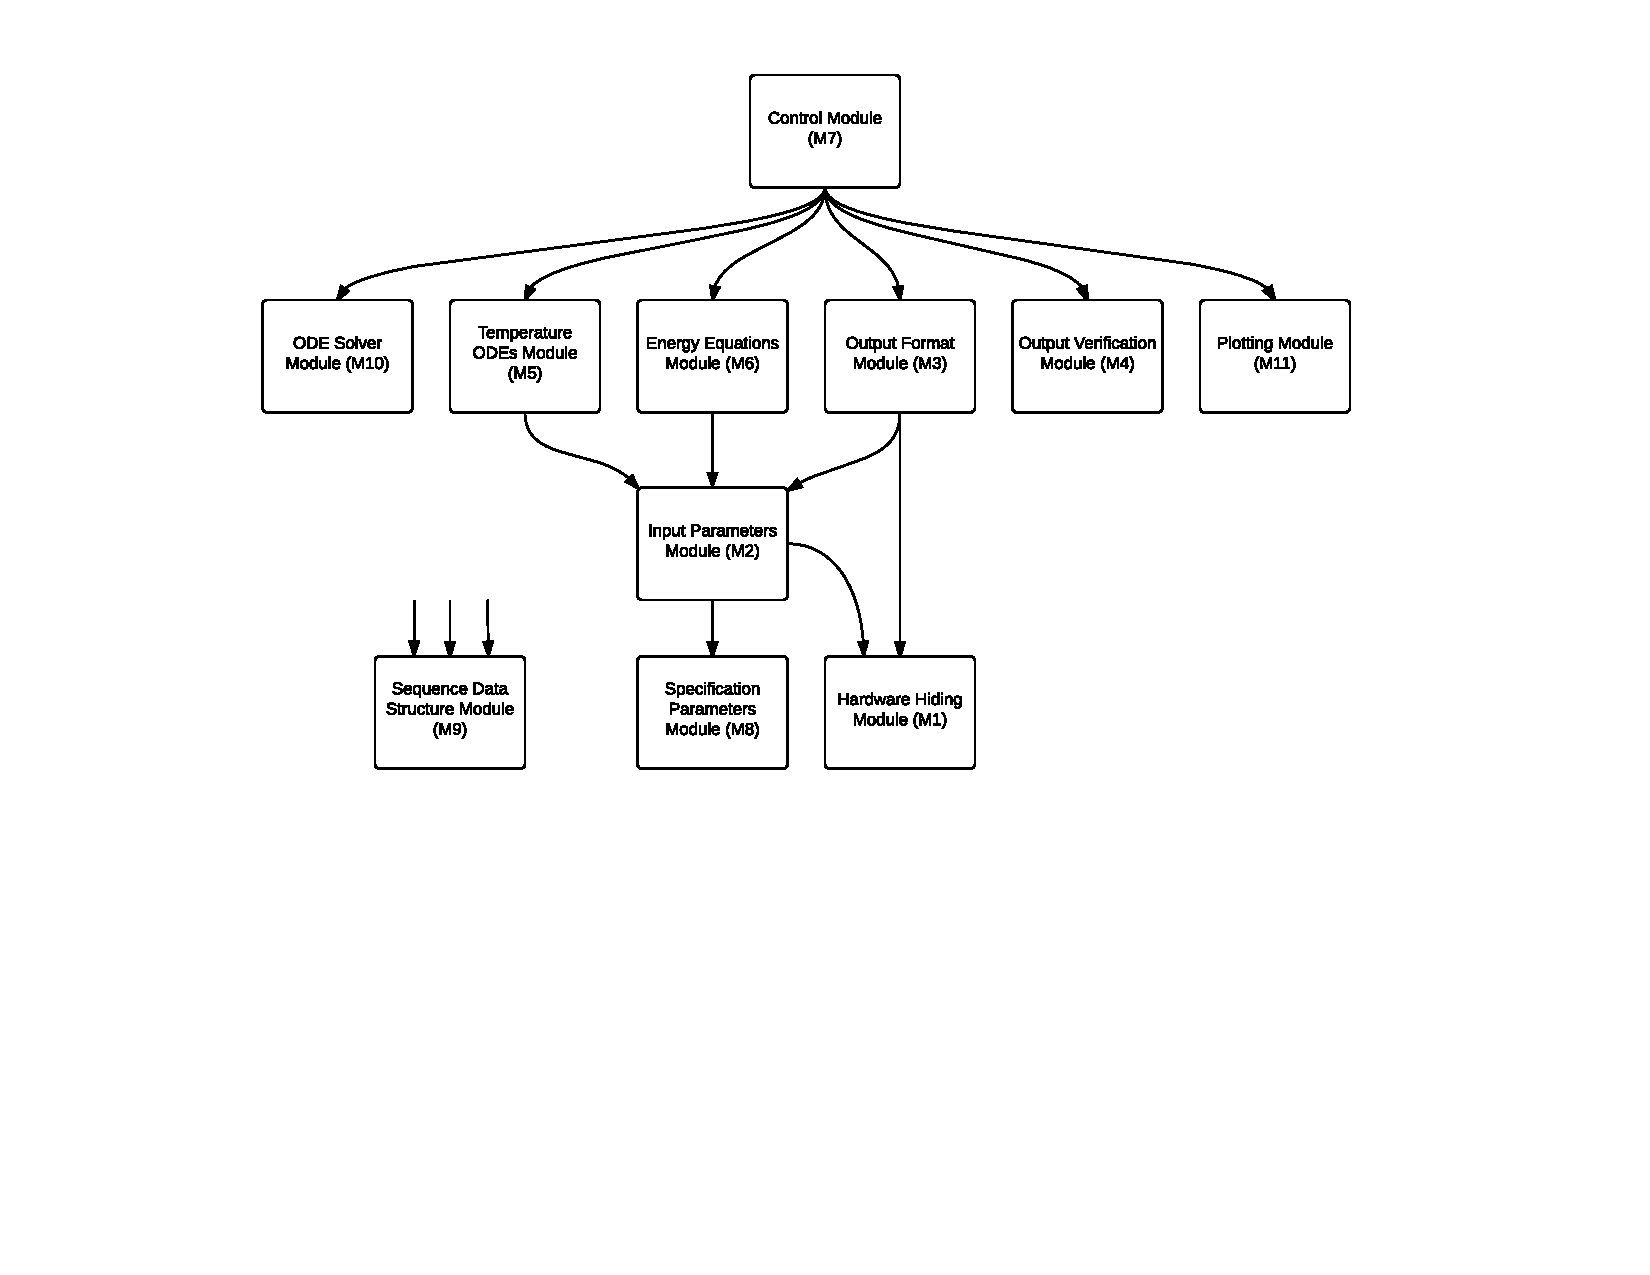
\includegraphics[scale=0.58]{../Figures/RevisedHierarchy.pdf}
\end{center}

\end{frame}

%%%%%%%%%%%%%%%%%%%%%%%%%%%%%%%%%%%%%%%%%%%%%%%%%%%%%%


\begin{frame}
\frametitle{Introduction}
\begin{itemize}
\item The material in these slides should hopefully be review, or
  reasonably easy to pick up
\item Shows the simple mathematics that can be used to build your MIS
\item Shows a syntax that you can use
\item The presentation follows \cite{HoffmanAndStrooper1995} (Chapter
  3) and \cite{GriesAndSchneider1993}
\end{itemize}
\end{frame}

%%%%%%%%%%%%%%%%%%%%%%%%%%%%%%%%%%%%%%%%%%%%%%%%%%%%%%

\begin{frame}
\frametitle{Sets, Relations and Functions}
\begin{itemize}
\item A set is an unordered collection of elements
\item A binary relation is a set of ordered pairs
\item A function is a relation in which each element in the domain
  appears exactly once as the first component in the ordered pair
\end{itemize}
\end{frame}

%%%%%%%%%%%%%%%%%%%%%%%%%%%%%%%%%%%%%%%%%%%%%%%%%%%%%%

\begin{frame}
\frametitle{Sets}
\begin{itemize}
\item An element either belongs to a set or it does not
\item $x \in S$ versus $x \notin S$
\item Defining a set
\begin{itemize}
\item Enumerate $\{ x_1, x_2, x_3, ..., x_n \}$
\item Logical condition (rule) $\{x | p(x) \}$
\item Notation from \cite{GriesAndSchneider1993} $\{x: X | R : E \}$
\item An integer range $[2 .. 4] = \{2, 3, 4\}$, $[7 .. 4] = \{\}$
\end{itemize}
\item Examples
\begin{itemize}
\item $S = \{ 1, 7, 6 \}$
\item $S = \{ x |$ $x$ is an integer between $1$ and $4$ inclusive
  $\}$
\item $S = \{ x: \mathbb{N} |$ $0 \leq x \leq 4$ : $x$ $\}$
%\item Clarify that there is no notion of ordering in sets
\end{itemize}
\item Does $\{ 1, 7, 6 \} = \{ 7, 1, 6 \}$?
\end{itemize}
\end{frame}

%%%%%%%%%%%%%%%%%%%%%%%%%%%%%%%%%%%%%%%%%%%%%%%%%%%%%%

\begin{frame}
\frametitle{Relations}
\begin{itemize}
\item Let $<x, y>$ denote an ordered pair
\begin{itemize}
\item $dom(R) = \{x | <x, y> \in R\}$
\item $ran(R) = \{y | <x, y> \in R\}$
\end{itemize}
\item Defining a relation
\begin{itemize}
\item Enumerate $\{ <0, 1>, <0, 2>, <2, 3> \}$
\item Rule $\{ <x, y>|$ $x$ and $y$ are integers and $x < y \}$
\item $\{ x, y: \mathbb{N} |$ $x < y$ : $<x, y> \}$
\end{itemize}
\end{itemize}
\end{frame}

%%%%%%%%%%%%%%%%%%%%%%%%%%%%%%%%%%%%%%%%%%%%%%%%%%%%%%

\begin{frame}
\frametitle{Functions}
\begin{itemize}
\item Let $<x, y>$ denote an ordered pair
\item Each element of the domain is associated with a unique element
  of the range
\item Defining a function
\begin{itemize}
\item Enumerate $\{ <0, 1>, <1, 2>, <2, 3> \}$
\item Rule $\{ <x, y> |$ $x$ and $y$ are integers and $y = x^2 \}$
\end{itemize}
\item Notation
\begin{itemize}
\item $f(a) = b$ means $<a, b> \in f$
\item $f(x) = x^2$
\item $f: T_1 \rightarrow T_2$
\item $\{ <<x_1, x_2>, y> |$ $x_1$, $x_2$ are integers and $y = x_1 + x_2 \}$
\end{itemize}
\item Is $\{ <0, 1>, <0, 2>, <2, 3> \}$ a function?
\item Is $\{ <x, y> |$ $x$ and $y$ are integers and $y^2 = x\}$?
\end{itemize}
\end{frame}

%%%%%%%%%%%%%%%%%%%%%%%%%%%%%%%%%%%%%%%%%%%%%%%%%%%%%%

\begin{frame}
\frametitle{Logic}
\begin{itemize}
\item A logical expression is a statement whose truth values can be
  determined ($6 < 7$?)
\item Truth values are either \emph{true} or \emph{false}
\item Complex expressions are formed from simpler ones using logical
  connectives ($\neg$, $\wedge$, $\vee$, $\rightarrow$,
  $\leftrightarrow$)
\item Truth tables
\item Evaluation
\begin{itemize}
\item Decreasing order of precedence: $\neg$, $\wedge$, $\vee$,
$\rightarrow$, $\leftrightarrow$
\item Evaluate from left to right
\item Use rules of boolean algebra
\end{itemize}
\end{itemize}
\end{frame}

%%%%%%%%%%%%%%%%%%%%%%%%%%%%%%%%%%%%%%%%%%%%%%%%%%%%%%

\begin{frame}
\frametitle{Quantifiers}
\begin{itemize}
\item Variables are often used inside logical expressions
\item Variables have types
\item A type is a set of values from which the variable can take its value
\item Often quantify a logical expression over a given variable
\begin{itemize}
\item Universal quantification
\item Existential quantification
\end{itemize}
\end{itemize}
\end{frame}

%%%%%%%%%%%%%%%%%%%%%%%%%%%%%%%%%%%%%%%%%%%%%%%%%%%%%%

\begin{frame}
\frametitle{Quantifiers Continued}

\begin{itemize}
\item Prefer \cite[p.\ 143]{GriesAndSchneider1993} notation for quantification
  (and set building)
\item $(*x: X | R : P)$ means application of the operator $*$ to the values $P$ for
all $x$ of type $X$ for which range $R$ is true.  In the above equations, the
$*$ operators include $\forall$, $\exists$ and $+$ are used
\item Example on next slide for rank function specification
\end{itemize}

\end{frame}

%%%%%%%%%%%%%%%%%%%%%%%%%%%%%%%%%%%%%%%%%%%%%%%%%%%%%%

\begin{frame}
%\frametitle{Quantifiers Example for Rank Function}

\noindent $\mbox{rank}(a, A): \mathbb{R} \times \mathbb{R}^n \rightarrow \mathbb{R}$\newline
$\mbox{rank}(a, A) \equiv \mbox{avg}(\mbox{indexSet}(a, \mbox{sort}(A)))$\newline

\noindent $\mbox{indexSet}(a, B): \mathbb{R} \times \mathbb{R}^n \rightarrow \mbox{ set of }
\mathbb{N}$\newline
$\mbox{indexSet}(a, B) \equiv \{j: \mathbb{N} | j \in [1..|B|]
\wedge B_j = a : j \}$\newline

\noindent $\mbox{sort}(A): \mathbb{R}^n \rightarrow \mathbb{R}^n$\newline
$\mbox{sort}(A) \equiv B: \mathbb{R}^n, \mbox{ such that }$\newline
$\forall (a: \mathbb{R} | a \in A : \exists(b: \mathbb{R} | b \in B: b = a)
\wedge \mbox{count}(a, A) = \mbox{count}(b, B)) \wedge \forall (i: \mathbb{N} | i \in [1..|A|-1] : B_i \leq B_{i+1})$\newline

\noindent $\mbox{count}(a, A): \mathbb{R} \times \mathbb{R}^n \rightarrow \mathbb{N}$\newline
$\mbox{count}(a, A): + (x: \mathbb{R} | x \in A \wedge x = a : 1)$\newline

\noindent $\mbox{avg}(C): \mbox{ set of } \mathbb{N} \rightarrow \mathbb{R}$\newline
$\mbox{avg}(C) \equiv + (x: \mathbb{N} | x \in C : x) / |C|$\newline

\end{frame}

%%%%%%%%%%%%%%%%%%%%%%%%%%%%%%%%%%%%%%%%%%%%%%%%%%%%%%

\begin{frame}
\frametitle{Quantifiers Continued}
\begin{itemize}
\item Bound variables appear in the scope of the quantifier
\item Free variables are not bound to any quantifier
\item Free variables in an expression often  mean that we cannot determine the truth value of the expression
\end{itemize}
\end{frame}

%%%%%%%%%%%%%%%%%%%%%%%%%%%%%%%%%%%%%%%%%%%%%%%%%%%%%%

\begin{frame}
\frametitle{Types, Sets, Sequence and Tuples}
\begin{itemize}
\item A type is a set of values, so any precisely defined set is a type
\item Primitive types are often integer, boolean, character, string
  and real
\item Types can include functions ($T_1 \rightarrow T_2$)
\item User-defined types
\begin{itemize}
\item The set of values has to be given
\item Often use type constructors
\end{itemize}
\item Useful type constructors
\begin{itemize}
\item Set
\item Sequence
\item Tuple
\end{itemize}
\end{itemize}
\end{frame}

%%%%%%%%%%%%%%%%%%%%%%%%%%%%%%%%%%%%%%%%%%%%%%%%%%%%%%

\begin{frame}
\frametitle{Types}
\begin{itemize}
\item Specify the type of a variable
\begin{itemize}
\item $x_1, x_2, ..., x_n : T$
\item $x: integer$
\item $a, b, c: string$
\end{itemize}
\item Type definition
\begin{itemize}
\item $T = d$
\item $float = real$
\item $colour = \{red, white, blue \}$
\item $testtype = \{uniaxial, biaxial, shear \}$
\item $x: testtype$
\item $motionT = \{ forward, backward, stop \}$
\end{itemize}
\end{itemize}
\end{frame}

%%%%%%%%%%%%%%%%%%%%%%%%%%%%%%%%%%%%%%%%%%%%%%%%%%%%%%

\begin{frame}
\frametitle{Primitive Types}
\begin{itemize}
\item Integer
\begin{itemize}
\item $\{ ... -2, -1, 0, 1, 2, ... \}$
\item $+, -, \times, /$
\item $=, \neq$
\item $<, \leq, \geq, >$
\end{itemize}
\item Real
\begin{itemize}
\item $\{ all~real~numbers \}$
\item $+, -, \times, /, \sin (), \cos (), \exp ()$ etc.
\item $=, \neq$
\item $<, \leq, \geq, >$
\end{itemize}
\end{itemize}
\end{frame}

%%%%%%%%%%%%%%%%%%%%%%%%%%%%%%%%%%%%%%%%%%%%%%%%%%%%%%

\begin{frame}
\frametitle{Primitive Types Continued}
\begin{itemize}
\item Boolean type
\begin{itemize}
\item $\{ true, false \}$
\item $\neg$, $\wedge$, $\vee$, $\rightarrow$, $\leftrightarrow$
\end{itemize}
\item Char type
\begin{itemize}
\item Set of ASCII characters
\item Character values appear in quotes $'a'$, $'b'$, $'c'$, etc.
\item $=, \neq$
\end{itemize}
\end{itemize}
\end{frame}

%%%%%%%%%%%%%%%%%%%%%%%%%%%%%%%%%%%%%%%%%%%%%%%%%%%%%%

\begin{frame}
\frametitle{Primitive Types Continued}
\begin{itemize}
\item String type
\begin{itemize}
\item All finite sequences of characters
\item String constants are in double quotes $''abc''$
\item $s[i..j]$ is the substring of $s$ from position $i$ to position $j$
\item $s_1 || s_2$ concatenates strings $s_1$ and $s_2$
\item $=, \neq$ for is equal and not equal
\item $\in, \notin$ for is member and not a member
\item $s[i]$ is the $i$th character of $s$
\item $|s|$ is the length of $s$
\item Positions in strings are zero relative
\end{itemize}
\end{itemize}
\end{frame}

%%%%%%%%%%%%%%%%%%%%%%%%%%%%%%%%%%%%%%%%%%%%%%%%%%%%%%

\begin{frame}
\frametitle{Sets}
\begin{itemize}
\item A set is an unordered collection of elements of the same type
\item Declare a set of type $T$ as $set~of~T$
\item Example
\begin{itemize}
\item $T = set~of~ \{red, green, blue \}$ defines type $T$ as the power set of $\{red, green, blue \}$
\item $x: set~of~integer$
\end{itemize}
\item What are some possible values for $x: set~of~integer$?
\end{itemize}
\end{frame}

%%%%%%%%%%%%%%%%%%%%%%%%%%%%%%%%%%%%%%%%%%%%%%%%%%%%%%

\begin{frame}
\frametitle{Operations on Sets}
\begin{itemize}
\item $\cup$ union
\item $\cap$ intersection
\item $-$ difference
\item $\times$ Cartesian product
\item $=, \neq$ equal, not equal
\item $\in, \notin$ member, non-member
\item $|s|$ size of set $s$
\end{itemize}
\end{frame}

%%%%%%%%%%%%%%%%%%%%%%%%%%%%%%%%%%%%%%%%%%%%%%%%%%%%%%

\begin{frame}
\frametitle{Sequences}
\begin{itemize}
\item A sequence is an ordered collection of elements of the same type
\begin{itemize}
\item Elements can occur more than once
\item Sometimes referred to as a list
\item Similar to an array
\end{itemize}
\item Declare a sequence of type $T$ by $sequence~of~T$
\item $< x_0, x_1, ..., x_n >$ for $n \geq 0$ for a sequence with elements $x_0, x_1, ..., x_n$
\item $< >$ is the empty sequence
\item Position in a sequence is zero relative
\end{itemize}
\end{frame}

%%%%%%%%%%%%%%%%%%%%%%%%%%%%%%%%%%%%%%%%%%%%%%%%%%%%%%

\begin{frame}
\frametitle{Sequences Continued}
\begin{itemize}
\item Examples
\begin{itemize}
\item $T = sequence~of~\{ red, green, blue \}$ defines the type $T$ as the set of all sequences of elements from
$\{red, green, blue \}$
\item $x: sequence~of~integer$
\end{itemize}
\item Fixed-length sequence of type $T$ with length $l$
\begin{itemize}
\item $sequence~[l]~of~T$
\item $l$ is a positive integer
\item $sequence~[l_1, l_2, ..., l_n ]~of~T$ is a shorthand for $sequence~[l_1]~of~sequence~[l_2]~of ... sequence~
[l_n]~ of~T$
\end{itemize}
\end{itemize}
\end{frame}

%%%%%%%%%%%%%%%%%%%%%%%%%%%%%%%%%%%%%%%%%%%%%%%%%%%%%%

\begin{frame}
\frametitle{Operations on Sequences}
\begin{itemize}
\item $s[i..j]$ is the subsequence of $s$ from position $i$ to position $j$
\item $s[i..j]$ is undefined if $i \notin [0..|s|-1] \vee j \notin [0 .. |s|-1]$
\item $s_1 || s_2$ concatenates sequences $s_1$ and $s_2$
\item $=, \neq$ for is equal and not equal
\item $\in, \notin$ for is member and not a member
\item $s[i]$ is the $i$th element of $s$
\item $s[i]$ is undefined if $i \notin [0..|s|-1]$
\item $|s|$ is the length of $s$
\item A string is a sequence of characters
\end{itemize}
\end{frame}

%%%%%%%%%%%%%%%%%%%%%%%%%%%%%%%%%%%%%%%%%%%%%%%%%%%%%%

\begin{frame}
\frametitle{Tuples}
\begin{itemize}
\item A tuple is a collection of elements of possibly different types
\item Each tuple has one or more fields
\item Each field has a unique identifier called the field name
\item Similar to a record or a structure
\item To declare a tuple use
\begin{itemize}
\item $tuple~of~(f_1: T_1, f_2: T_2, ..., f_n: T_n )$ with $n \geq 1$
\item $f_i$ is the name of the $i$th field
\item $T_i$ is the type of the $i$th field
\item $tuple~of~(f_1, f_2, ..., f_n: T )$ if all fields are of the same type
\end{itemize}
\end{itemize}
\end{frame}

%%%%%%%%%%%%%%%%%%%%%%%%%%%%%%%%%%%%%%%%%%%%%%%%%%%%%%

\begin{frame}
\frametitle{Example Tuples}
\begin{itemize}
\item Examples
\begin{itemize}
\item $pair = tuple~of~(id: integer, val: string)$
\item $experimentT = tuple~of~(b_{cond}: bcondT, control: controlT)$
\end{itemize}
\item Define the value of a tuple by using an expression of the form
\begin{itemize}
\item $<x_1, x_2, ..., x_n >$
\item $<4, ''cat''>$ is a value of type pair
\end{itemize}
\end{itemize}
\end{frame}

%%%%%%%%%%%%%%%%%%%%%%%%%%%%%%%%%%%%%%%%%%%%%%%%%%%%%%

\begin{frame}
\frametitle{Operations on Tuples}
\begin{itemize}
\item $=, \neq$ equal, not equal
\item $t.f$ is the value of field $f$ of tuple $t$
\end{itemize}
\end{frame}

%%%%%%%%%%%%%%%%%%%%%%%%%%%%%%%%%%%%%%%%%%%%%%%%%%%%%%

\begin{frame}
\frametitle{Using Type Constructors}
\begin{itemize}
\item $bcondT = \{ uniaxial, biaxial, multiaxial, shear \}$
\item $controlT = \{ load\_controlled, displacement\_controlled \}$
\item $experimentT = tuple~of~(b_{cond}: bcondT, control: controlT)$
\item $experiment: experimentT$
\item $directionT = \{clockwise, counterclockwise \}$
\item $powerT = [MIN\_POWER ... MAX\_POWER]$
\item $motorT = tuple~of~ (powerOn: Boolean,~direction: directionT,~powerLevel: powerT)$
\end{itemize}
\end{frame}

%%%%%%%%%%%%%%%%%%%%%%%%%%%%%%%%%%%%%%%%%%%%%%%%%%%%%%

\begin{frame}
\frametitle{Multiple Assignment Statement}
\begin{itemize}
\item $v_1, v_2, ..., v_n := e_1, e_2, ...,, e_n$ with $n \geq 1$
\item The $v_i$s are distinct variables and each $e_i$ is an expression of the same type as $v_i$
\item Compute the values of all the expression $e_i$ and then assign these values simultaneously
\item Example
\begin{itemize}
\item $x, y := 0, 10$
\item $x, y := 10, x$
\item $x, y := y, x$
\end{itemize}
\item Convenient for defining the meaning of pieces of code
\item Use as a function on the state space of a program
\end{itemize}
\end{frame}

%%%%%%%%%%%%%%%%%%%%%%%%%%%%%%%%%%%%%%%%%%%%%%%%%%%%%%

\begin{frame}
\frametitle{Conditional Rules}
\begin{itemize}
\item $(c_1 \Rightarrow r_1 | ... | c_n \Rightarrow r_n )$, where $n \geq 1$
\item $c_i$s are the logical expressions
\item $r_i$s are the rules
\item $c_i \Rightarrow r_i$ is the $i$th component of the rule
\item The first $c_i$ that evaluates to true applies rule $r_i$
\item If no condition is true then the conditional rule is undefined
\end{itemize}
\end{frame}

%%%%%%%%%%%%%%%%%%%%%%%%%%%%%%%%%%%%%%%%%%%%%%%%%%%%%%

\begin{frame}
\frametitle{Uses of Conditional Rules}
\begin{itemize}
\item To define the value of a function
\item $min(x,y) = (x \leq y \Rightarrow x | x > y \Rightarrow y)$
\item To define the meaning of a program
\begin{itemize}
\item If $(x < y)$ then $z := x$ else $z := y$
\item $(x < y \Rightarrow z := x | x \geq y \Rightarrow z:= y)$
\item $(x < y \Rightarrow x, y := x, y | x \geq y \Rightarrow x, y := y, x)$
\end{itemize}
\item Conditional rules can be expressed in tables
\end{itemize}
\end{frame}

%%%%%%%%%%%%%%%%%%%%%%%%%%%%%%%%%%%%%%%%%%%%%%%%%%%%%%

\begin{frame}
\frametitle{Finite State Machines}
\begin{itemize}
\item A FSM is a tuple $(S, s_0, I, O_E, O_O, T, E, C)$ where
\item $S$ is a finite set of states
\item $s_0$ is the initial state in $S$ $(s_0 \in S)$
\item $I$ is a finite set of inputs
\item $T: S \times I \rightarrow S$ is the transition function
\item $O_E$ is a finite set of event outputs
\item $E: S\times I \rightarrow O_E$ is the event output
\item $O_C$ is a finite set of condition outputs
\item $C: S \rightarrow O_C$ is the condition output
\end{itemize}
\end{frame}

%%%%%%%%%%%%%%%%%%%%%%%%%%%%%%%%%%%%%%%%%%%%%%%%%%%%%%

\begin{frame}[allowframebreaks]
\frametitle{References}

\bibliography{../../ReferenceMaterial/References}

\end{frame}

%%%%%%%%%%%%%%%%%%%%%%%%%%%%%%%%%%%%%%%%%%%%%%%%%%%%%%

\end{document}